\subsection{Il Palladio}\label{palladio}
Data la potenza dei motori di ricerca odierni, si verifica spesso il fenomeno del \textit{deep linking}: l'utente non entra nel sito tramite la Home Page, ma viene "catapultato" in una pagina interna in seguito ad un ricerca. È quindi importante offrire all'utente alcune informazioni che lo aiutino ad orientarsi. \\
Verrà quindi analizzata la pagina \\ \url{https://itstecnologie.it/index.php/il-palladio/}.\\ Le foto presenti risalgono a giugno 2018.

\IMG{"Pagina Il Palladio 1"}
\IMG{"Pagina Il Palladio 2"}
\IMG{"Pagina Il Palladio 3"}
\IMG{"Pagina Il Palladio 4"}

\subsubsection{Assi Informativi Obbligatori}
\paragraph{What} 
Nulla di diverso da segnalare rispetto alla Home Page. Il logo in alto a sinistra contiene un link alla Home Page, e a metà della pagina vi è una descrizione di alcuni servizi offerti.
\paragraph{Who}
Nessuna differenza da quanto riportato per la Home Page.
\paragraph{Where}
Nulla di molto diverso dalla Home Page per quanto riguarda la prima vista (figura \ref{"Pagina Il Palladio 1"}). Una grande immagine sopra la quale scorrono delle parole "d'effetto" ma prive di contenuto concreto. Una miglioria rispetto alla Home Page è l'assenza della metafora visiva del pulsante e la presenza di una immagine che rappresenta un prodotto dell'azienda anche se, per un utente che non conosce tale prodotto, rimane priva di significato, risultando in spazio sprecato. \\ Il logo è l'unica cosa che risponde a questo asse, ma come detto per la Home Page l'assenza di un ulteriore testo esplicativo non aiuta a capire dove si è giunti. Con uno scroll si può capire che l'azienda lavora in un settore legato alla casa, con pavimenti, arredo bagno, caminetti e wellness e servizi collegati. \\
Sorprende in modo negativo l'assenza di breadcrumbs: nessuna indicazione sulla nostra posizione all'interno del sito, generando un spiacevole senso di disorientamento. Come sono arrivato a questa pagina? Come posso approfondire le informazioni che ho cercato? O come posso tornare ad un livello precedente per cercare informazioni diverse ma collegate? La mancanza di breadcrumb non permette la risposta a queste domande, rendendo la navigazione e la ricerca delle informazioni più complicata.

\subsubsection{Assi Informativi Opzionali}

\paragraph{When}
Nessuna differenza rispetto alla Home Page: rimangono le critiche già fatte.
\paragraph{Why}
Nessun particolare sforzo posto per offrire informazioni a riguardo. Come si vede in figura \ref{"Pagina Il Palladio 2"} vi è una descrizione dei servizi svolti, ma nulla che spinga il cliente a rimanere sul sito o a non scegliere la concorrenza.
\IMG{Pulsanti}
\paragraph{How}
Anche qui per navigare sono presenti il menu e la funzionalità di ricerca, come per la Home Page. Tramite appositi link è possibile approfondire determinati argomenti o scaricare cataloghi. Nota negativa dei pulsanti presenti (figura \ref{Pulsanti}) è la parola "scopri" che li caratterizza: un parola priva di contenuto, che non indica all'utente dove andrà una volta cliccato il pulsante. La presenza di una parola al di sopra del pulsante attutisce questo effetto negativo, ma se per problemi di layout i pulsanti dovessero spostarsi, la loro destinazione non sarebbe affatto chiara. Sorprende come si sia scelto di rendere cliccabili sia il pulsante che il testo sopra con animazioni diverse: potrebbe far sorgere il dubbio di arrivare a due destinazioni diverse in seguito al click. \\
La presenza in fondo dei contatti e della mappa offre ulteriori strumenti di comunicazione all'utente (figura \ref{"Pagina Il Palladio 3"} e \ref{"Pagina Il Palladio 4"}).

\IMG{Pavimenti}

\subsection{Pavimenti e rivestimenti}
La pagina in questione (figura \ref{Pavimenti}) è raggiungibile all'indirizzo \\ \url{https://itstecnologie.it/index.php/pavimenti-e-rivestimenti/}, e all'interno del sito è raggiungibile unicamente dalla pagina "Il Palladio" trattata nella sezione \ref{palladio}. \\ Essendo la struttura uguale alla pagina precedente non vi sono critiche aggiuntive da fare per quanto riguarda gli assi informativi, ma sono presenti alcuni elementi degni di nota che si presentano anche in altre pagine.

\subsubsection{Breadcrumb}
\IMG{Breadcrumb}
Come si era potuto capire dall'analisi della pagina precedente, in questo sito il breadcrumb è molto sottovalutato: qui è presente, ma indica che la pagina precedente è la Home Page (figura \ref{Breadcrumb}). Ciò è indice di una disorganizzazione interna del sito come anticipato nella sezione \ref{struttura}. \\
Per giungere a questa pagina devo necessariamente passare per la pagina Il Palladio, presente nel menu, e non per la Home Page. Risulta così complicato per l'utente ritornare sui propri passi e recuperare le informazioni di cui necessita.

\subsubsection{Immagini}
L'azienda utilizza il sito per inserire alcune immagini dei propri lavori, e assumono così un ruolo importante. In questa pagina notiamo che la dimensione scelta per le immagini è di 380x380 pixel, rispettando la taglia minima consigliata di 210x230 pixel. \\La scelta di disporre le immagini a griglia permette di usare bene lo spazio, evitare troppi scroll e semplificare la navigazione.
Al passaggio del mouse appare una scritta che specifica a cosa si riferisce la foto, che risulta cliccabile. \\
Un'effe to migliore si sarebbe ottenuto distanziando leggermente le immagini, evitando così una sensazione di sovraccarico della pagina. \\ Si segnala che ciò è implementato nella pagina N-Touch all'url= \url{https://itstecnologie.it/index.php/ntouch/}, così da avere un paragone delle due tecniche (figura \ref{"Dettaglio Griglia N-Touch"}).
\IMG{"Dettaglio Griglia N-Touch"}
Per completezza, analizzo brevemente la "galleria" che si apre cliccando su un'immagine, in particolare quella all'url \url{https://itstecnologie.it/index.php/portfolio/particolari-cantieri-abitazioni-ns-clienti/}. \\
Come si vede dalla figura \ref{Galleria} il layout è abbandonato a se stesso. Vi sono delle brevi frasi all'inizio della pagina che non hanno nessun collegamento con le foto e si riferiscono a servizi generici dell'azienda. Le immagini sono disposte in un ordine quasi privo di logica: è stata abbandonata la struttura a griglia precedente e vengono disposte in due colonne, con quella di destra molto più lunga. Si costringe l'utente a fare numerosi scroll per vedere tutto, e le immagini offerte non sono cliccabili o visualizzabili in dettaglio, ma statiche. Generalmente l'utente è abituato che in seguito al click su un'immagine accada qualcosa, ma qui ciò non è permesso, impattando negativamente sull'esperienza di navigazione dell'utente. \\
\\ Da notare che il breadcrumb è nuovamente sparito.

\begin{figure}[H]
	\centering
	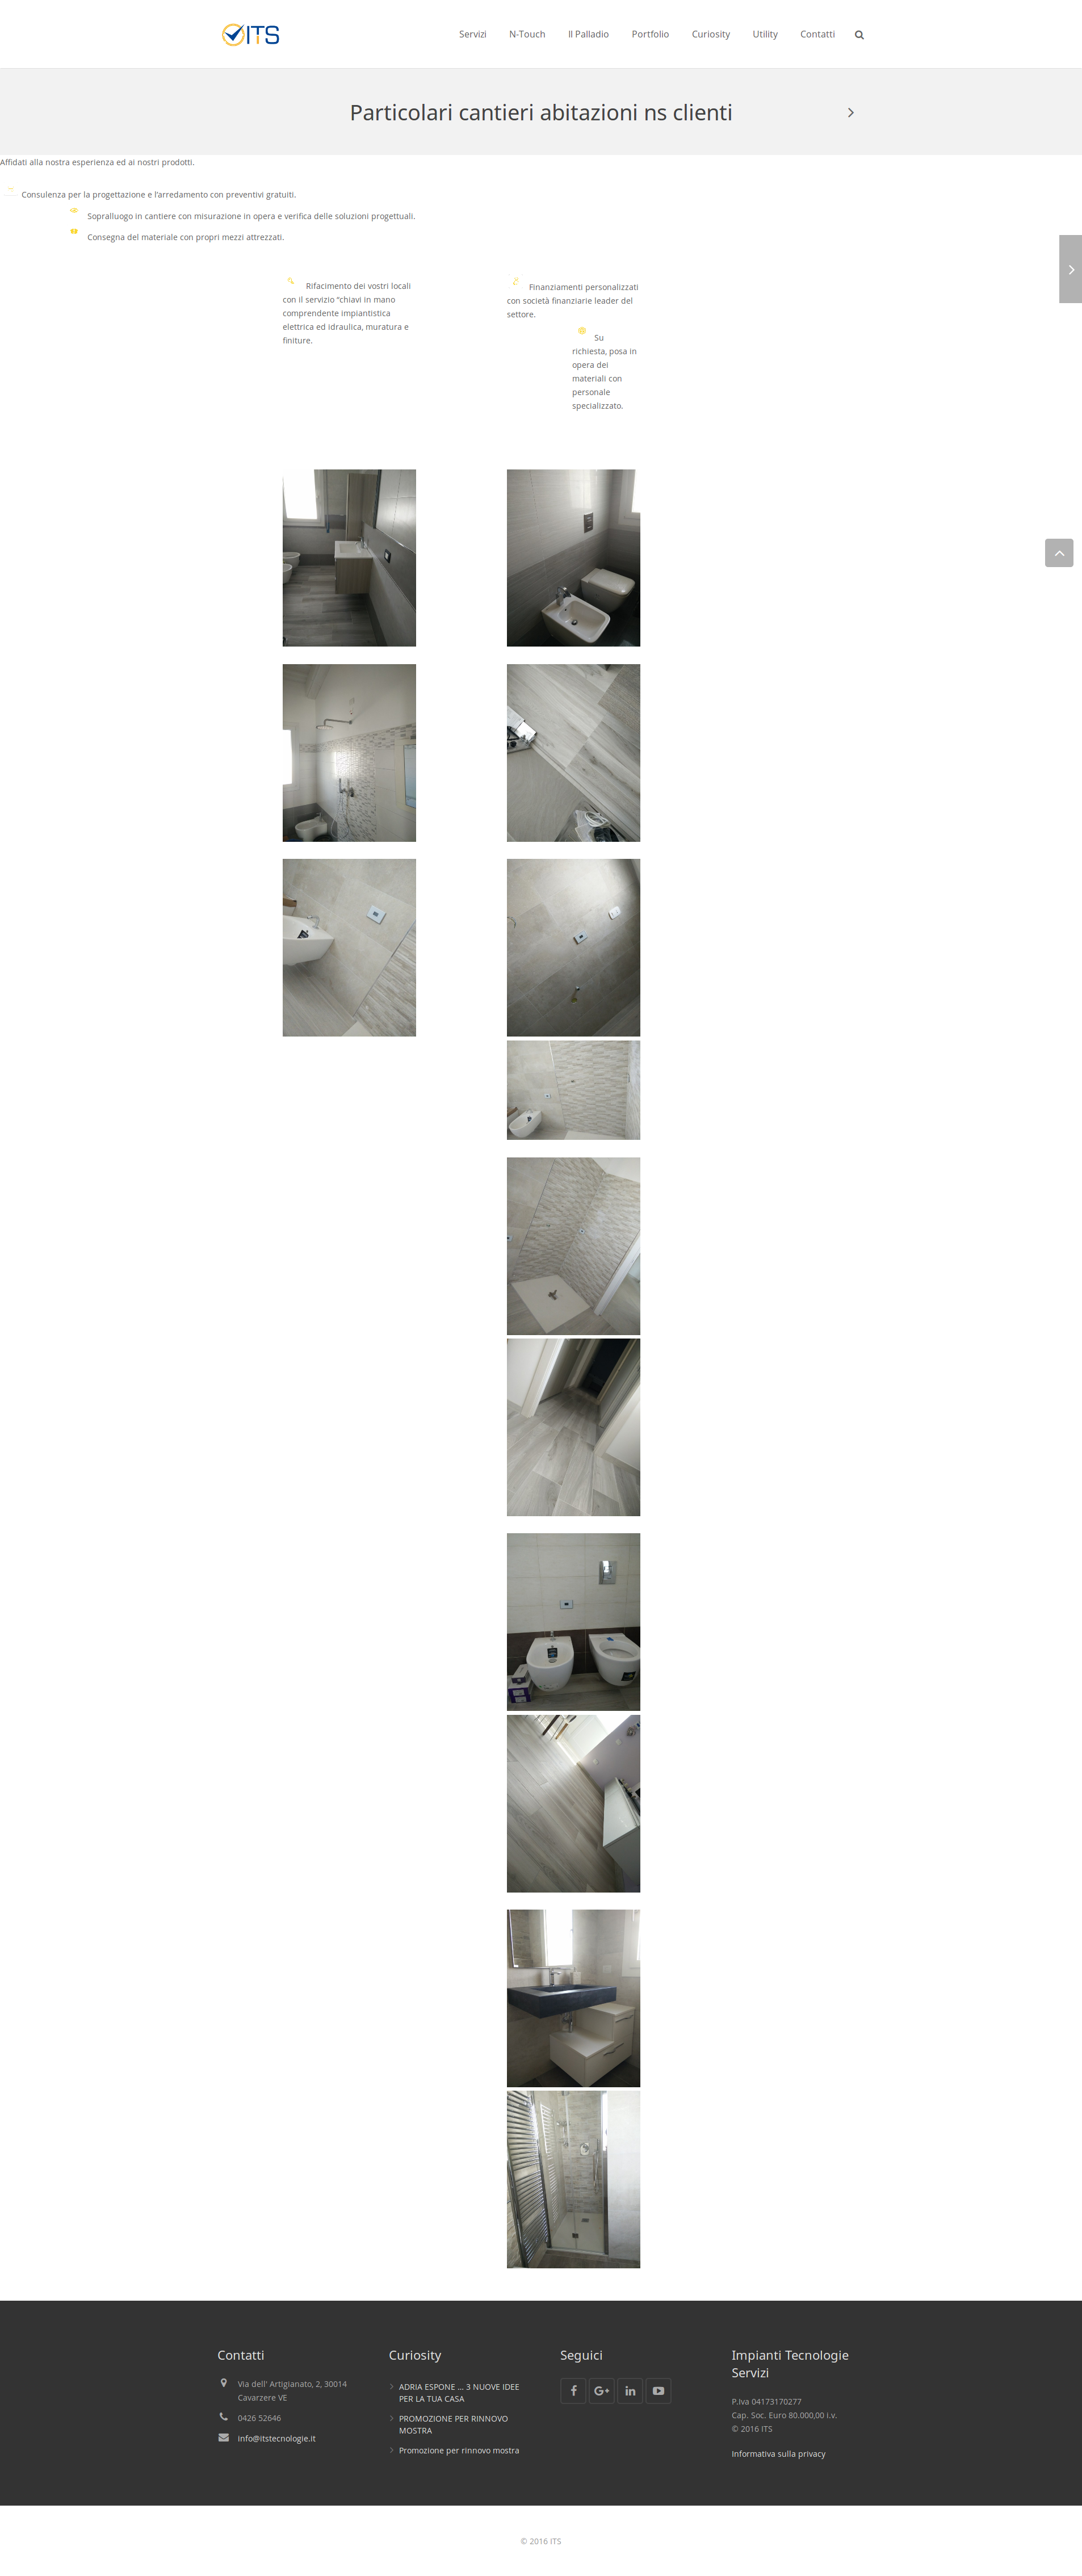
\includegraphics[width=\textwidth,height=\textheight,keepaspectratio]{img/Galleria.png}
	\caption{Galleria fotografica}\label{Galleria}
\end{figure}

\subsubsection{Conenuto}
Gli utenti navigano perchè sono alla ricerca di contenuti, principalmente testuali. Il sito sottovaluta anche quest'aspetto: nella pagina in analisi non vi è nessuna informazione testuale, se non in accompagnamento delle foto, e nella galleria quel poco testo che c'è è disorganizzato e completamente scollegato al resto del contenuto. \\ Si segnala, per confronto, che il contenuto è più curato e organizzato nella pagina \url{https://itstecnologie.it/index.php/ntouch/} (figura \ref{"Dettaglio Contenuto N-Touch"}), anche se: \begin{itemize}
\item le dimensioni del font, \item l'uso di caratteri maiuscoli sul titolo, \item la distribuzione in griglia, \item la compattezza del testo \item la mancanza di parole chiave evidenziate \end{itemize} rendono la lettura poco piacevole.

\IMG{"Dettaglio Contenuto N-Touch"}
